%%%%%%%%%%%%%%%%%%%%%%%%%%%%%%%%%%%%%%%%%
% Template
% LaTeX Template
% Version 1.0 (December 8 2014)
%
% This template has been downloaded from:
% http://www.LaTeXTemplates.com
%
% Original author:
% Brandon Fryslie
% With extensive modifications by:
% Vel (vel@latextemplates.com)
%
% License:
% CC BY-NC-SA 3.0 (http://creativecommons.org/licenses/by-nc-sa/3.0/)
%
% Authors:
% Sabbir Ahmed, Jeffrey Osazuwa, Howard To, Brian Weber
% 
%%%%%%%%%%%%%%%%%%%%%%%%%%%%%%%%%%%%%%%%%

\documentclass[paper=usletter, fontsize=12pt]{article}
%%%%%%%%%%%%%%%%%%%%%%%%%%%%%%%%%%%%%%%%%
% Contract
% Structural Definitions File
% Version 1.0 (December 8 2014)
%
% Created by:
% Vel (vel@latextemplates.com)
% 
% This file has been downloaded from:
% http://www.LaTeXTemplates.com
%
% License:
% CC BY-NC-SA 3.0 (http://creativecommons.org/licenses/by-nc-sa/3.0/)
%
%%%%%%%%%%%%%%%%%%%%%%%%%%%%%%%%%%%%%%%%%

%----------------------------------------------------------------------------------------
%   PARAGRAPH SPACING SPECIFICATIONS
%----------------------------------------------------------------------------------------

\setlength{\parindent}{0mm} % Don't indent paragraphs

\setlength{\parskip}{2.5mm} % Whitespace between paragraphs

%----------------------------------------------------------------------------------------
%   PAGE LAYOUT SPECIFICATIONS
%----------------------------------------------------------------------------------------

\usepackage{geometry} % Required to modify the page layout
\usepackage{multicol}

\setlength{\textwidth}{16cm} % Width of the text on the page
\setlength{\textheight}{23cm} % Height of the text on the page

\setlength{\oddsidemargin}{0cm} % Width of the margin - negative to move text left, positive to move it right

% Uncomment for offset margins if the 'twoside' document class option is used
%\setlength{\evensidemargin}{-0.75cm} 
%\setlength{\oddsidemargin}{0.75cm}

\setlength{\topmargin}{-1.25cm} % Reduce the top margin

%-------------------------------------------

\usepackage[utf8]{inputenc} % Required for including letters with accents
\usepackage[T1]{fontenc} % Use 8-bit encoding that has 256 glyphs

\usepackage{avant} % Use the Avantgarde font for headings
\usepackage{mathptmx} % Use the Adobe Times Roman as the default text font together with math symbols from the Sym­bol, Chancery and Com­puter Modern fonts

%----------------------------------------------------------------------------------------
%   SECTION TITLE SPECIFICATIONS
%----------------------------------------------------------------------------------------

\usepackage{titlesec} % Required for modifying section titles

\titleformat{\section} % Customize the \section{} section title
{\sffamily\large\bfseries} % Title font customizations
{\thesection} % Section number
{16pt} % Whitespace between the number and title
{\large} % Title font size
\titlespacing*{\section}{0mm}{7mm}{0mm} % Left, top and bottom spacing around the title

\titleformat{\subsection} % Customize the \subsection{} section title
{\sffamily\normalsize\bfseries} % Title font customizations
{\thesubsection} % Subsection number
{16pt} % Whitespace between the number and title
{\normalsize} % Title font size
\titlespacing*{\subsection}{0mm}{5mm}{0mm} % Left, top and bottom spacing around the title
\renewcommand\familydefault{\sfdefault} % specifies the document layout and style

%-----------------------------------------------------------------------------

% names
\newcommand{\team}{Galois Field Arithmetic Unit}
\newcommand{\Sabbir}{Sabbir Ahmed}
\newcommand{\Jeffrey}{Jeffrey Osazuwa}
\newcommand{\Howard}{Howard To}
\newcommand{\Brian}{Brian Weber}

% document info command
\newcommand{\documentinfo}[5]{
    \begin{centering}
        \parbox{2in}{
        \begin{spacing}{1}
            \begin{flushleft}
                \begin{tabular}{l l}
                    #1 \\
                    #2 \\
                    #3 \\
                    #4 \\
                    #5 \\
                \end{tabular}\\
                \rule{\textwidth}{1pt}
            \end{flushleft}
        \end{spacing}
        }
    \end{centering}
}

\begin{document}


    \documentinfo
    {\textbf{MEMO NUMBER:} GFAU\_SRS\_01}
    {\textbf{DATE:} \today}
    {\textbf{TO: } EFC LaBerge}
    {\textbf{FROM: }\Sabbir, \Jeffrey, \Howard, \Brian}
    {\textbf{SUBJECT: } System Requirement Specifications Draft}
    \vspace{-0.1in}

    \section{Introduction}
    A Galois field is a field with a finite number of elements. The nomenclature $GF(q)$ is used to indicate a Galois field with q elements. For $GF(q)$ in general, $q$ must be a power of a prime. For each prime power, there exists exactly one finite field. The best known and most used Galois field is $GF(2)$, the binary field.

    The \team~ handles irreducible polynomials in $GF(2^n)$, where $\{2 \leq n \leq 16\}$. The ALU generates all the terms in the field of the polynomial, and allows the user to view and apply the following binary operations:

    \begin{itemize}

        \item Addition
        \item Subtraction
        \item Multiplication
        \item Division
        \item Logarithm

    \end{itemize}

        \subsection{Mission Scenario}
        Cryptography has many expensive calculations that are difficult for low power and inexpensive microcontrollers to handle. Galois fields are frequently used in the field of cryptography. The GFAU will make Galois field computations more accessible to such low powered devices.

        \subsection{Document Overview}
        This document serves as the System Requirements Specification for the Galois Field Arithmetic Unit. The description and requirements of the project are embodied in this document.

        The Specification is divided into separate segments pertaining to individual components and requirements on different levels. Figures and tables are attached where necessary to assist in demonstrating concepts.

        \section{System Overview}
        The GFAU system is composed of discrete modules residing in a single programmable board. Individual modules shall be programmed to solely complete an assigned task. Although modules are assigned individual tasks, they shall not have exclusive components for its functionality.

        \subsection{System Boundary Diagram}
        The system boundary diagram of the GFAU has been provided in Figure \ref{fig:system_boundary} below.

        \begin{figure}[ht]
            \begin{center}
                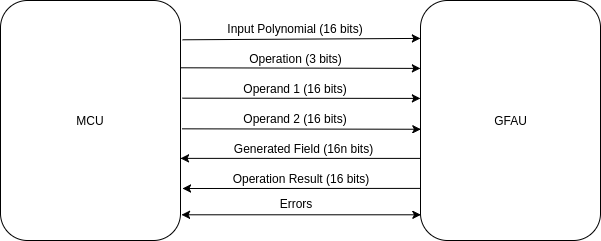
\includegraphics[width=1\textwidth]{system_boundary.png}
                \caption{System Boundary Diagram of the \team~, where $n$ is the Number of Terms} \label{fig:system_boundary}
            \end{center}
        \end{figure}

        The user input and output (I/O) interface are handled by the microcontroller (MCU) which are transferred via busses. The user inputs consist of the mode bit, the input generating polynomial and the binary operation(s) along with their corresponding operands. The MCU transfers the data to the unit to perform the desired operations. The GFAU will return the outputs and any errors detected back to the MCU.
        \newpage

        \subsection{Functional Flow Diagram}
        The functional flow diagram of the GFAU has been provided in Figure \ref{fig:functional_flow}.

        \begin{figure}[ht]
            \begin{center}
                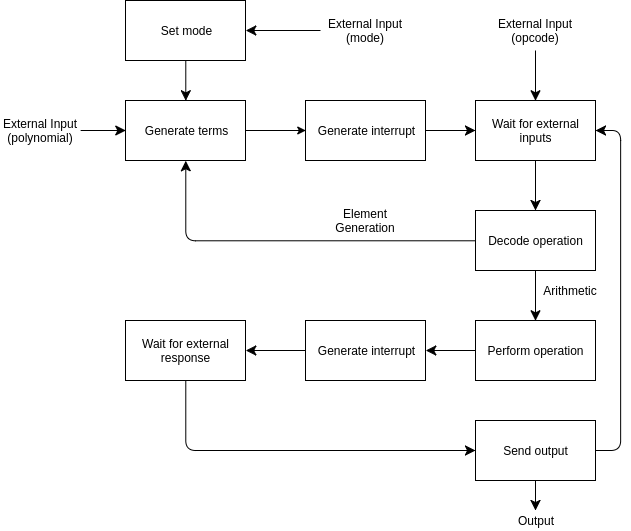
\includegraphics[width=1\textwidth]{functional_flow.png}
                \caption{Functional Flow Diagram of the \team~} \label{fig:functional_flow}
            \end{center}
        \end{figure}

        The diagram provides a high-level overview of the sequence of processes that take place in the unit. In total, the unit waits for an input from the user in three separate instances. The order of the inputs are essential for the unit to proceed as desired. The \textbf{mode} input sets the width of the data bus in the GFAU. The \textbf{polynomial} input consist of the generating polynomial to generate its terms in the Galois field. The \textbf{operation} input consists of the two operands along with the desired binary operation.
        \newpage

        \subsection{Data Flow Diagram}
        The data flow diagram of the GFAU has been provided in Figure \ref{fig:data_flow}.

        \begin{figure}[ht]
            \begin{center}
                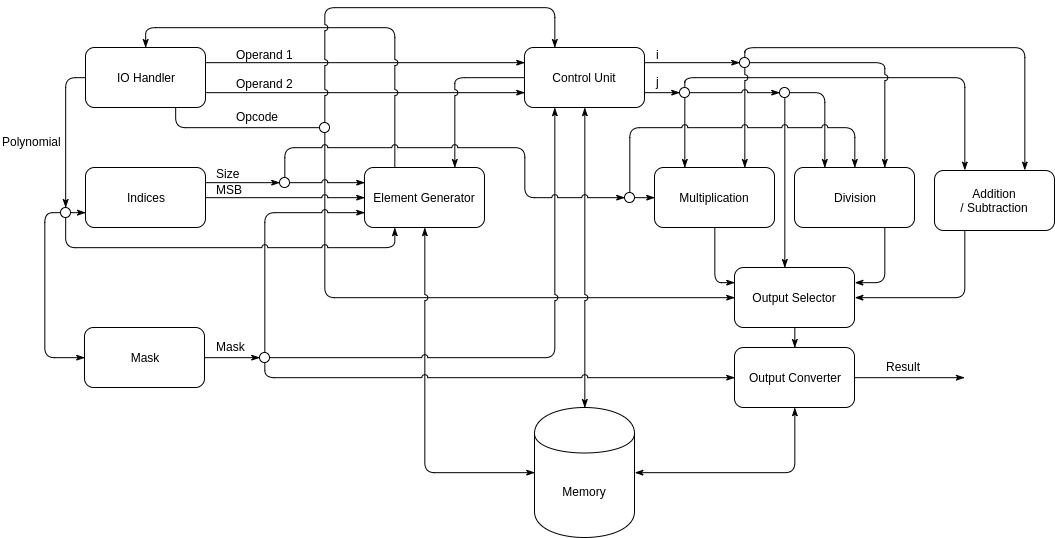
\includegraphics[width=1\textwidth]{data_flow.png}
                \caption{Data Flow Diagram of the \team~} \label{fig:data_flow}
            \end{center}
        \end{figure}

        The diagram provides a lower-level view of the system emphasizing the individual components and their role in converting the input data to the desired output. The \textbf{Error} lines are used by multiple components to send interrupt signals to the user when required.

    \section{Requirements}

        \subsection{Cost and Package Constraints}
        This section outlines all design constraints imposed by the customer, from which the remainder of the requirements are derived.

        \begin{enumerate}

            \item The total cost of the prototype shall not exceed \$400
            
            \item The total area of prototype printed circuit board (PCB) shall not exceed 24 inches square
            
            \item The cost at mass production shall not exceed \$1 per chip
            
            \item The package of the final product shall not exceed 64 pins and should use fewer than 64 pins.

        \end{enumerate}

        \subsection{Hardware Requirements}
        Hardware portability shall be prioritized on the GFAU. The hardware portability provides flexibility in the ranges of its specifications. The ranges of these specifications shall be reasonably bounded.

        \begin{enumerate}

            \item The unit shall be functional at a variety of clock speeds at a minimum range of [4 MHz - 100 MHz].

            \item The GFAU shall perform its computations in [0.5] instructions per clock cycle

            \item The GFAU shall not exceed a thermal design power (TDP) of [1] W

            \item The GFAU shall operate normally at a temperature range of -40$^{\circ}$C \textasciitilde 85$^{\circ}$C

            \item The input/draining? voltage for the unit shall be [5] V

        \end{enumerate}

        \subsection{Software and Testing Requirements}
        Extensive simulations shall be conducted during the development of the design in a hardware description language (HDL). This process makes debugging easier and minimizes the risk of unintended behavior in the prototype. This section outlines the HDL code requirements and tests that the simulations are required to pass.

        \begin{enumerate}

            \item Extensive design verification simulations shall be done before purchasing any hardware. The exact simulations shall be left up to the designer, however they shall prove the device operates as expected with at least a [99\%] probability. 

            \item All HDL code shall be synthesizable

            \item Gate delay and other relevant values shall be parametrized to easily match the specifications of candidate hardware during verification

        \end{enumerate}

        \subsection{Signal Testing and Requirements}
        To ensure that all communication occurs correctly between the external device and GFAU, all signals shall meet the rise and fall times outlined below. Additionally, this section describes which tools shall be used to verify the correctness of the output, and the tools that shall be used to verify the rise and fall times of each signal.

        \begin{enumerate}

            \item All output signals shall not exceed rise and fall times of [1 ns]
            
            \item All output signals rise and fall times shall be measured using an oscilloscope to verify they meet [1].
            
            \item All output shall be checked probabilistically using a digital logic analyzer.

        \end{enumerate}

        \subsection{Communication Requirements}
        In order for the GFAU to be able to communicated with a wide variety of external devices, the GFAU shall implement communication methods which are commonly used. The details of how the GFAU shall communicate are outlined in this section.

        \begin{enumerate}
            
            \item The GFAU shall have an option to use either a 8, 16, [or 32] bit data-bus.
            
            \item After any given operation is complete and the result is placed on the bus, the GFAU shall set a ready pin. 
            
            \item The external device may monitor the ready pin using polling or interrupts to know when to pull the data from the bus.
            
            \item The GFAU shall use a common or easy to implement protocol for pushing blocks of data over a bus that is too small to send on one clock.

        \end{enumerate}

            \subsubsection{Errors}
            This section outlines the cases in which errors are thrown.
            \begin{enumerate}

                \item The unit shall produce an error if an operand is not in the same Galois field.

                \item The unit shall produce an error if the FPGA does not receive all the inputs from the microcontroller.

                \item The microcontroller shall produce an error if it does not receive all the outputs from the FPGA.

            \end{enumerate}


\end{document}
